\documentclass[10pt]{article}
\usepackage[bottom=1.8in]{geometry} % see geometry.pdf on how to lay out the page. There's lots.
\geometry{a4paper} % or letter or a5paper or ... etc
% \geometry{landscape} % rotated page geometry

\author{Byron Vickers, Mike McKeown, Gecia Bravo Hermsdorff}
\title{Final Project Report \\ {\Large COS 424 Interacting with Data (2014)} }
\date{}

\usepackage{fullpage}
%\usepackage{byron}
\usepackage{fancyvrb}
\VerbatimFootnotes


\begin{document}

\maketitle

\section{Introduction}
We want to build a ranking of student enjoyment and satisfaction on graduate (PhD) programs at universities across the US. 

We want to do this for a couple of reasons: It's pretty entertaining, for one, but it's also valuable information for any prospective graduate student trying to decide where to apply, or which offers to accept. The current tools available for doing this are pretty limited: sites such as {\tt usnews.com} and {\tt forbes.com} offer little if any information on student satisfaction, while less formal ranking systems such as {\tt collegeprowler.com} (now moved to {\tt colleges.niche.com}) have sparse data and suffer from the bias problems inherent in any crowd sourced review system.

------------

As mentioned above, there are a number of review websites which offer partial data on student satisfaction in graduate programs. There are also several university-specific results on student satisfaction; internal surveys done by universities to gauge what they are doing well and what needs to be improved.\footnote{Some examples: \verb|http://www.utexas.edu/news/2011/12/01/grad_climate_study/|, \\
\verb|http://www.ohio.edu/education/news-and-events/upload/Final-2013-Student-Satisfaction-Report-8-23-13.pdf|,\\
\verb|http://ga.berkeley.edu/files/page/surveyreport.pdf|}

We would like to take a completely different approach to the problem: using sentiment analysis on the acknowledgment sections of submitted theses to try and gauge how satisfied students were at the point where they finish their degrees and are about to leave the university.

There are 3.6 million english PhD theses listed on \verb|proquest.com|. We propose to use a subset of these as our text corpus, most likely selecting a thousand or so from each of several top-ranked US universities. We will then extract the acknowledgments text from each thesis, run a (possibly made-from-scratch) sentiment analysis algorithm on it, and use these to build a profile of the university's student satisfaction.

While the rankings website data is useful as a sanity-check for our model (we expect our results to correlate strongly with the rankings, but probably not exactly), the university-commissioned student satisfaction surveys should give a good value for the ground-truth values, and we can use these to validate the predictive power of our algorithm. We can also use resources such as \verb|http://nlp.stanford.edu:8080/sentiment/rntnDemo.html| to check the performance of our sentiment analysis algorithm if we choose to develop one from scratch ourselves.

-----------

In attempting to rank university graduate programs based on student satisfaction, we would like to apply machine learning techniques to a text corpus consisting of dissertation acknowledgment sections from different universities.   We believe there will be a correlation between features of the dissertation acknowledgment sections and student satisfaction.  For example, if an acknowledgment is longer and more positive, it may indicate the student is more satisfied than terse acknowledgment sections.

We plan to explore a small collection of methods to extract university rankings based on the dissertation acknowledgments.  We will first need to extract features from the acknowledgments.  A couple features we have discussed already include the length of the acknowledgment section and the count of keywords in the text that may have a positive or negative connotation, however, there are probably others that we will explore as well.  The features could then be used individually to obtain some sort of score for each acknowledgment (in which an average for each university would result in a ranking) or could be aggregated for each university (based on all acknowledgments from the university) and obtain a ranking score for each university.

As for the machine learning algorithms, there are a number of different approaches to explore.  As mentioned previously, we could use sentiment analysis to obtain a score for how positive or negative an acknowledgment section is.  This would allow us to rank universities based on their average sentiment score.  Another possibility is to use a regression to determine a score for each acknowledgment or university.  We could also use a binary classifier to determine if a given acknowledgment is better than another and use this information to determine a score for an acknowledgment or university.  

There are also machine learning algorithms specifically tailored toward ranking, such as Ranking SVM, Bayes Rank, etc.  While we have not done too much research into how these algorithms work and the assumptions they make yet, we plan to do so in determining which ones we will explore.  In short, there are many data analysis techniques that can be applied to this problem, and we intend to explore a subset of them that make valid assumptions about our problem and match up with the type of data we have and our goal.

\section{Data Collection}
The theses used for our analysis were taken from the ProQuest Full Text Thesis and Dissertation Database\footnote{Searchable via \texttt{http://search.proquest.com/pqdtft/}}. This database contains 1.5 million theses, when doing searches for English-language documents with full text available. The database includes metadata specifying features such as date of submission, University, Department, subject, and so on. All of this is freely available to licensed users -- notably, any user whose requests originates from within the IP block of a subscribing university (such as Princeton).

The data collection occurred in two stages: collecting the theses, and then running a parsing and extraction routine on them to pull out the text of the acknowledgements section.  Figure~\ref{fig:data_collect_block_diagram} shows a block diagram of this data collection process.

\begin{figure}
	\centering
	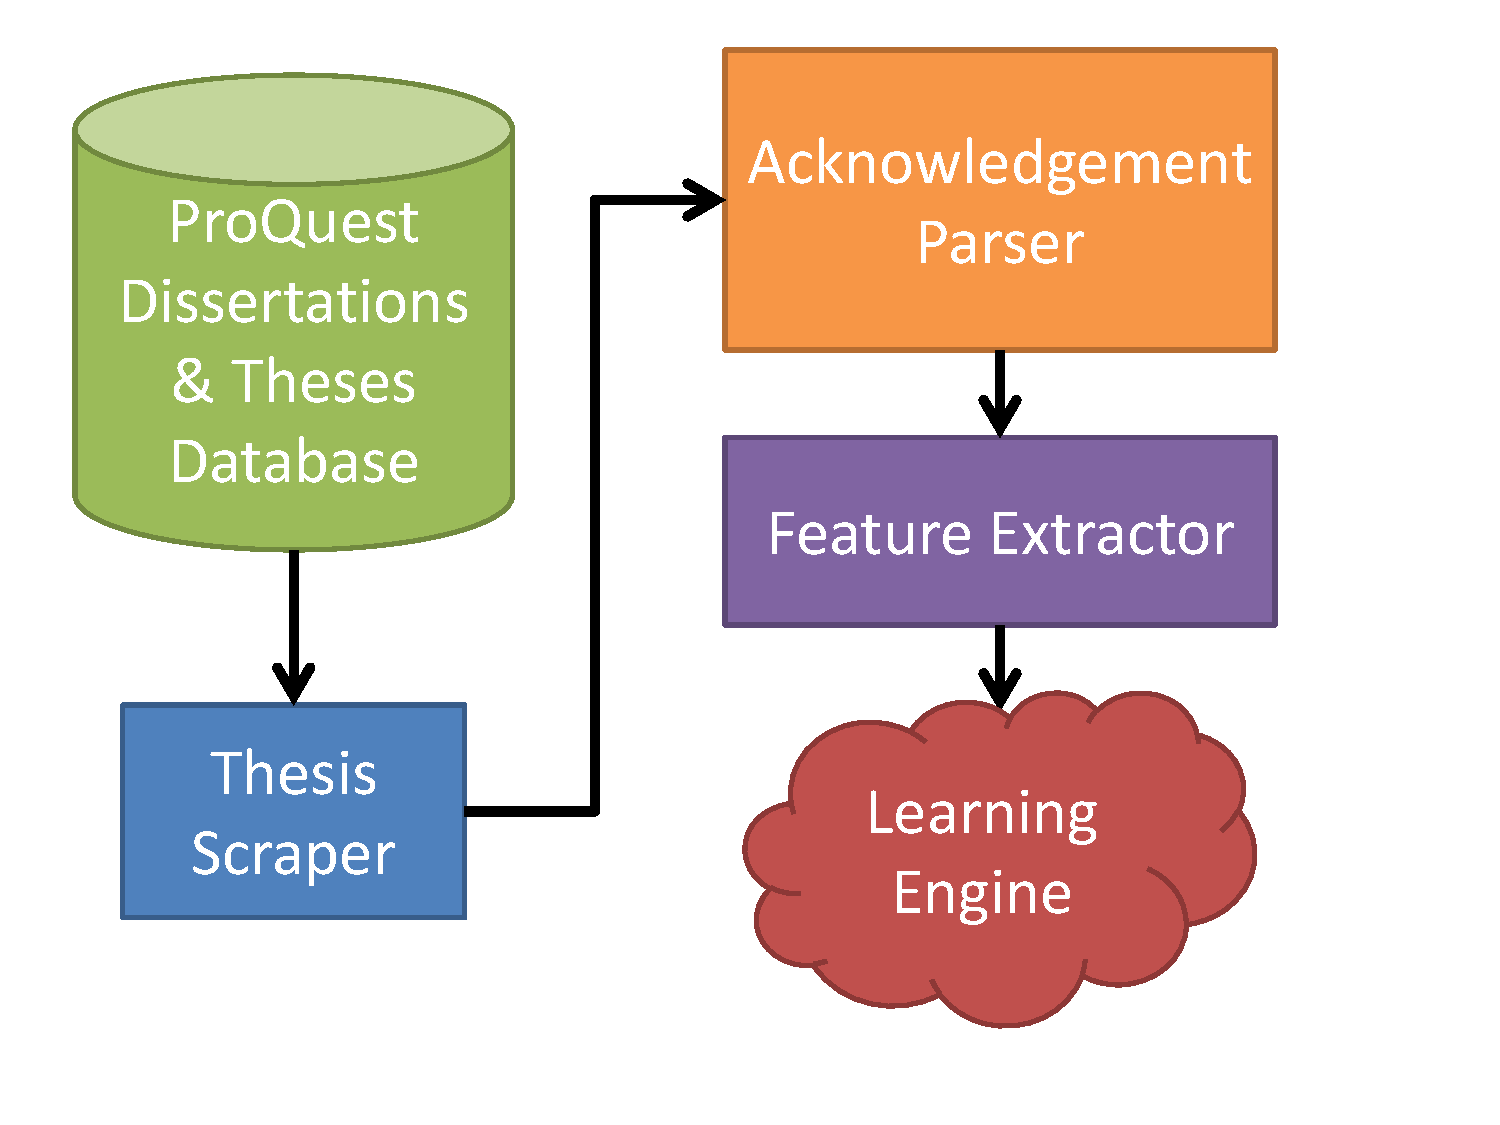
\includegraphics[width=0.5\textwidth]{block_diagram}
	\caption{Block diagram showing the data collection process}
	\label{fig:data_collect_block_diagram}
\end{figure}

\subsection*{Collecting theses (scraping)}
ProQuest has a database API exposed at \texttt{http://fedsearch.proquest.com/}. This access point seems to accept SRU (Search/Retrieval via URL)\footnote{See \texttt{http://www.loc.gov/standards/sru/}} queries, but fails to respond to the standard \texttt{Explain} operation, thus making its valid query terms unaccessible. Documentation for the service appears to be non-existent.\footnote{Though one user reports the existence of a document available from ProQuest on request: see \texttt{bibwild.wordpress.com/a-proquest-platform-api/}. He claims it is not very explanatory.}

We were successful in reverse-engineering the API to the extent where we could collect 1000 URLs of fulltext English theses. This is the dataset we went on to use for an analysis of PhD satisfaction by state over the United States. However, this dataset was insufficient for any analysis of individual universities.

At this point we switched to scraping documents via the standard, human-facing ProQuest search interface. When queries are made through this interface, ProQuest attempts to authenticate the humanity of the downloader using captcha-gateways for any downloads beyond a small number. Via various subterfuges, however, we were able to circumvent these measures and download 200 theses for each of the Ivy League universities.\footnote{The number 200 was chosen mainly to keep data processing times reasonable. With enough time (or compute power), our method should be easily extensible to at least several thousand theses per university} These form our second dataset.

Throughout this stage of the collection process we made extensive use of the Python packages \texttt{requests} and \texttt{BeautifulSoup} for HTTP requests and HTML parsing respectively.

\subsection*{Feature Extraction}

After scraping the PDFs and metadata for each thesis, the next task, as shown in Figure~\ref{fig:data_collect_block_diagram}, was to parse out the acknowledgement section.  This proved to be a more challenging task than we originally thought, thus, we had to resort to ad-hoc methods for identifying the location of the acknowledgement section within the PDF.

We extract the text from the PDF using \texttt{pdftotext}, which comes standard with the Xpdf\footnote{http://www.foolabs.com/xpdf/download.html} package in most linux installations.  This was the most robust solution we found in comparison with some Python PDF parsing libraries.  The output from \texttt{pdftotext} is a text file with the extracted text from the PDF.  The next task was to identify the acknowledgement section and parse it out.

Identifying the acknowledgement sections boiled down to identifying headings in the PDF.  Headings always occured on their own line and were relatively short.  When analyzing the text for headings, all page breaks, numbers, and punctuation were removed.  In addition, all the characters were converted to lower-case and all whitespace was removed.  This left headings on a single line and removed variation in capitalization, numbering of sections, etc.  

After identifying headings, it was trivial to find the start of the acknowledgements section, just look for the word acknowledgements (in practice I had to use some variations of acknowledgement, as there were some typos in this heading as well as spelling difference, such as "acknowledgment" versus "acknowledgement").  The removing of whitespace and other distracting characters avoided the case of identifying the acknowledgements listing in the table of contents as the actual acknowledgement section for most cases.  However, for some cases, we had to check that the acknowledgement heading and the terminating heading did not occur on the same page, as this would indicate we most likely found the table of contents.  The more difficult part was finding where the acknowledgement section ended.  Here we had to resort to going through many PDFs and finding common sections that follow the acknowledgement section.  This included "Table of Contents, "Abstract", "Dedication", "Introduction", etc.  Then we simply looked for these headings to identify where the acknowledgement section ended.  This allowed us to parse the large majority of acknowledgement sections, although we may miss a few that use non-standard headings or sections following the acknowledgement sections.

There were a couple caveats to parsing the acknowledgement section.  First, if the thesis had no acknowledgements section, the text returned would be empty.  This is exactly what we want, as we still wanted to include theses without acknowledgements in our data since the fact the student didn't write an acknowledgement section may say something about their satisfaction.  Second, if we found the acknowledgements section heading, but did not find a terminating heading after 5 pages of the PDF, we gave up and dropped that thesis from our data set.  This case indicates that we most likely missed the terminating heading (did not include it in our set of headings following the acknowledgement sections), since acknowledgement sections are generally less than 5 pages.  

The next step, as shown in Figure~\ref{fig:data_collect_block_diagram}, is to extract features from the acknowledgement section text.  This step was rather trivial.  We first converted all the characters to lower case, removed line and page breaks, removed digits, removed punctuation, and removed some odd UTF-8 characters that were parsed out of the PDF.  We then split all the words by whitespace, leaving us with an array of words in Python.  We used the Python Natural Language Toolkit\footnote{http://www.nltk.org/} (nltk) to remove stopwords and perform stemming.  We then converted this to a bag of words, i.e. list of counts for each word occuring in the document.  We returned the bag of words and total word count for analysis.

\section{Data Analysis}
How we analysed the data, once we had it out of the PDFs and into R.

Models we used (gaussian emission, and naive bayes). Issues with implementing the models.

\section{Results}
In addition to the results of the models discussed above, we can look at some summary statistics of the data to give us some insight into the plight of graduate students across the US.

Firstly, we can look at total number of thesis submissions on the ProQuest Thesis and Dissertation Database. This is shown in Figure~\ref{fig:pub_theses}.

\begin{figure}[H]
  \centering
  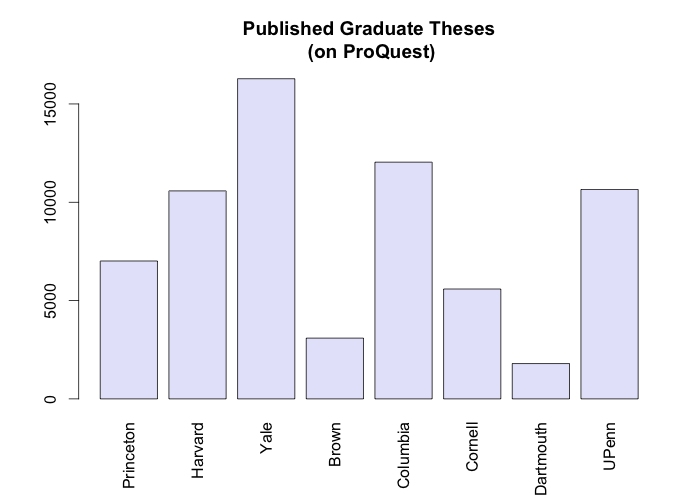
\includegraphics[width=0.5\textwidth]{img/pub_theses.png}
  \caption{Number of published graduate theses in ProQuest database}
  \label{fig:pub_theses}
\end{figure}

In Figure~\ref{fig:ack_lengths}, we can see that acknowledgement lengths drop off according to something akin to a power law, with a median length of around 400 words.

\begin{figure}[H]
  \centering
  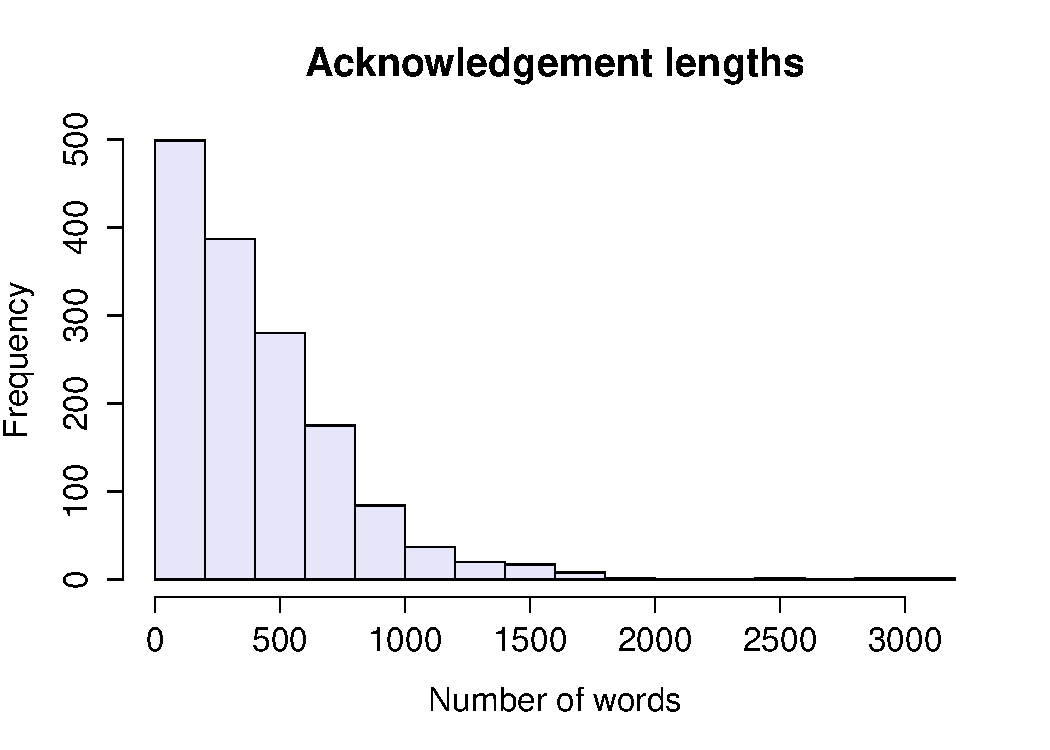
\includegraphics[width=0.5\textwidth]{img/ack_lengths.pdf}
  \caption{Acknowledgement lengths in graduate theses}
  \label{fig:ack_lengths}
\end{figure}

Examining the results of our models, we the table of fitted values for the university-conditional Gaussian positivity model is shown in Figure~\ref{fig:gaussian_model}. This provides one a plausible ranking of Ivy League universities by student satisfaction. Note, however, that the standard deviation of each university's positivity ratio is comparable to the inter-university positivity ratio differences, meaning that we cannot claim this ordering is statistically significant. This suggests that we may need to subclass the data within universities (by department, or field, most likely) in order to get clearer results. While the number of documents we collected was insufficient for this purpose, it would only be a matter of time and patience to collect a substantially larger corpus with which to work.

\begin{figure}[hH]
  \centering
  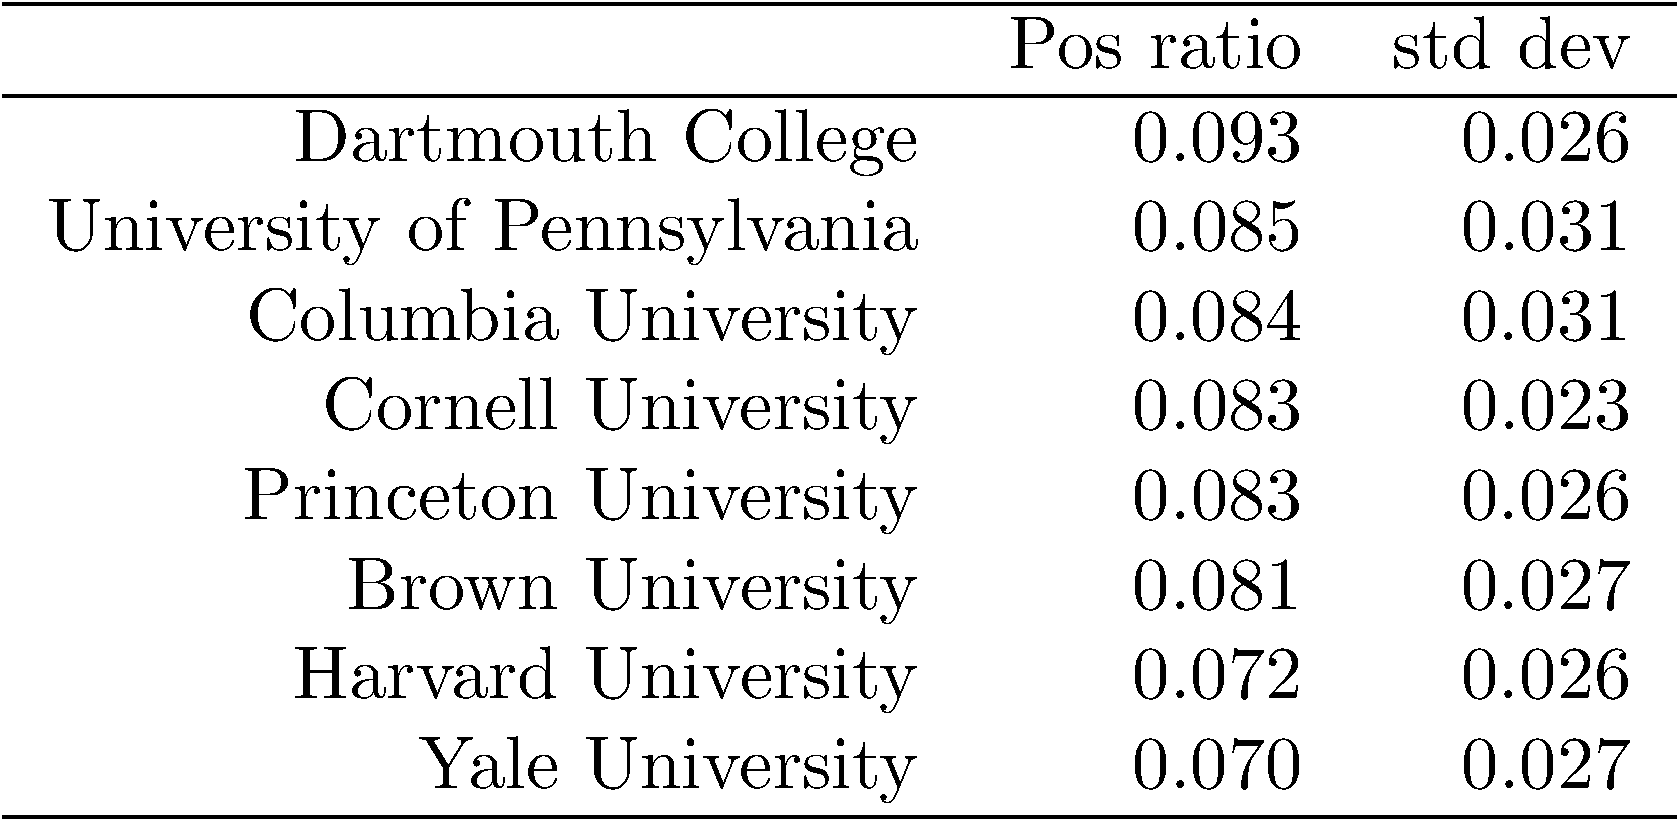
\includegraphics[width=0.5\textwidth]{img/gaussian_model.pdf}
  \caption{Fitted parameters to the university-conditional Gaussian positivity model}
  \label{fig:gaussian_model}
\end{figure}

The Naive Bayes classifier gave an accuracy of 72\% in predicting whether a student would fall in the top or bottom 50\% of positivity ratios, given the z-scored values for the university, the field (either biomedical sciences, humanities or sciences), the total number of negative words and the word count. The confusion matrix for the Naive Bayes classifier is included in Figure~\ref{fig:conf_matrix}.

\begin{figure}[hH]
  \centering
  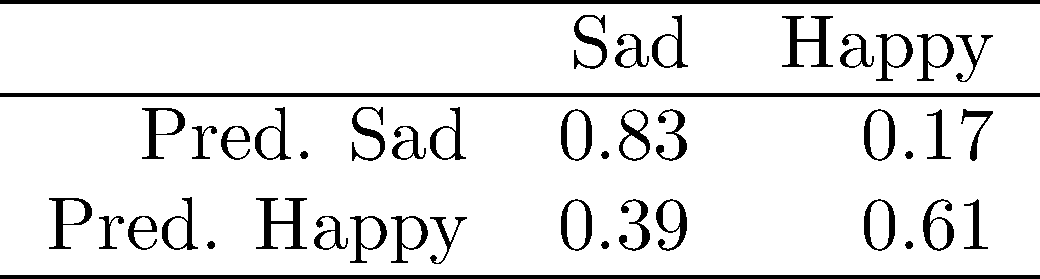
\includegraphics[width=0.5\textwidth]{img/conf_matrix.pdf}
  \caption{Confusion matrix for Naive Bayes classifier. Categories correspond to top and bottom 50\% of positivity ratios.}
  \label{fig:gaussian_model}
\end{figure}

Lastly, the rankings of positivity by field were:
\begin{enumerate}
  \item Sciences (mean 8.4\% positivity ratio)
  \item Biomedical sciences (mean 8.3\% positivity ratio)
  \item Humanities (mean 7.6\% positivity ratio)
\end{enumerate}
It is an open question as to whether these inter-subject differences are affected by differences in thesis conventions between subject areas.

\section{Conclusion}
Our project was a success as far as data collection and feature extraction. These areas were much mroe complex than we had anticipated them being, but in the end we were quite successful in building a text corpus with associated metadata.

Our analyses returned interesting results, but ultimately further investigation would need to be done in order to give strong conclusions. A thorough validation of the link between positivity in acknowledgement and student exit-satisfaction is also required -- an obvious way to go about this would be to individually contact students who have recently submitted and survey them on satisfaction, but such a procedure is outside the scope of this project. On the text-analysis side, an interesting question would be to see what other information can be gleaned from an analysis of the acknowledgement (or other sections of the PhD); we had hoped to perform such an analysis but were stymied by lack of time.

In conclusion, it seems there is reasonable evidence that acknowledgement sections can give insights into student satisfactions, and quite probably information well beyond this. This area could benefit from further research.

\section{References}

Bing Liu, Minqing Hu and Junsheng Cheng. "Opinion Observer: Analyzing  and Comparing Opinions on the Web." Proceedings of the 14th International World Wide Web conference (WWW-2005), May 10-14,  2005, Chiba, Japan.

Bing Liu. "Sentiment Analysis and Subjectivity." An chapter in  Handbook of Natural Language Processing, Second Edition, (editors: N. Indurkhya and F. J. Damerau), 2010.

Monroe, B., Colaresi, M., and Quinn, K. 2008. "Fightin' words: Lexical feature selection and evaluation for identifying the content of political conflict". Political Anal. 16, 4, 372--403.

Minqing Hu and Bing Liu. "Mining and Summarizing Customer Reviews." Proceedings of the ACM SIGKDD International Conference on Knowledge  Discovery and Data Mining (KDD-2004), Aug 22-25, 2004, Seattle,Washington, USA





\section{Appendices?}

\end{document}














